% !TEX program = lualatex

\documentclass[English,Chinese,French,JP,TC,use boldface,simple name]{beaulivre}

%%================================
%% Import toolkit
%%================================
\usepackage{ProjLib}
\usepackage{longtable}  % breakable tables
% \usepackage{hologo}     % more TeX logo
\usepackage{subfig}
\usetikzlibrary{calc}
\graphicspath{{../fig}}

\UseLanguage{Chinese}

\usepackage{varwidth}
\newtcolorbox{warning}[1][]{enhanced,
  before skip=2mm,after skip=3mm,
  boxrule=0.4pt,left=5mm,right=2mm,top=1mm,bottom=1mm,
  colback=yellow!50,
  colframe=yellow!20!black,
  sharp corners,rounded corners=southeast,arc is angular,arc=3mm,
  underlay={%
    \path[fill=tcbcolback!80!black] ([yshift=3mm]interior.south east)--++(-0.4,-0.1)--++(0.1,-0.2);
    \path[draw=tcbcolframe,shorten <=-0.05mm,shorten >=-0.05mm] ([yshift=3mm]interior.south east)--++(-0.4,-0.1)--++(0.1,-0.2);
    \path[fill=yellow!50!black,draw=none] (interior.south west) rectangle node[white]{\Huge\bfseries !} ([xshift=4mm]interior.north west);
    },
  drop fuzzy shadow,#1}
\newtcolorbox{advice}[2][]{enhanced,skin=enhancedlast jigsaw,
  attach boxed title to top left={xshift=-4mm,yshift=-0.5mm},
  fonttitle=\bfseries\sffamily,varwidth boxed title=0.7\linewidth,
  colbacktitle=blue!45!white,colframe=red!50!black,
  interior style={top color=blue!10!white,bottom color=red!10!white},
  boxed title style={
    empty,arc=0pt,outer arc=0pt,boxrule=0pt},
    underlay boxed title={
    \fill[blue!45!white] (title.north west) -- (title.north east)
    -- +(\tcboxedtitleheight-1mm,-\tcboxedtitleheight+1mm)
    -- ([xshift=4mm,yshift=0.5mm]frame.north east) -- +(0mm,-1mm)
    -- (title.south west) -- cycle;
    \fill[blue!45!white!50!black] ([yshift=-0.5mm]frame.north west)
    -- +(-0.4,0) -- +(0,-0.3) -- cycle;
    \fill[blue!45!white!50!black] ([yshift=-0.5mm]frame.north east)
    -- +(0,-0.3) -- +(0.4,0) -- cycle; },
title={#2},#1}

%%================================
%% For typesetting code
%%================================
\usepackage{listings}
\definecolor{maintheme}{RGB}{70,130,180}
\definecolor{forestgreen}{RGB}{21,122,81}
\definecolor{lightergray}{gray}{0.99}
\lstset{
  keywordstyle=\color{maintheme},
  basicstyle=\ttfamily,
  commentstyle=\color{forestgreen}\ttfamily,
  stringstyle=\color{violet}\ttfamily,
  showstringspaces=false,
  breaklines=true,
  frame=lines,
  backgroundcolor=\color{lightergray},
  columns=fixed,
  escapeinside={(*}{*)},
  numbers=left,
  numberstyle=\scriptsize, stepnumber=1, numbersep=5pt,
  % firstnumber=last,
  morekeywords={
      std, cout, endl
  }
}
\lstdefinestyle{v} % Verilog style
{
  language=Verilog,
  keywordstyle=\color{maintheme},
  basicstyle=\ttfamily,
  commentstyle=\color{forestgreen}\ttfamily,
  stringstyle=\color{violet}\ttfamily,
  showstringspaces=false,
  breaklines=true,
  frame=lines,
  backgroundcolor=\color{lightergray},
  columns=fixed,
  escapeinside={(*}{*)},
  numbers=left,
  numberstyle=\scriptsize, stepnumber=1, numbersep=5pt,
  % firstnumber=last,
  morekeywords={
      std, cout, endl
  }
  moredelim=*[s][\colorIndex]{[}{]},
  literate=*{:}{:}1
}
\definecolor{vorange}{RGB}{255,143,102}
\makeatletter
\newcommand*\@lbracket{[}
\newcommand*\@rbracket{]}
\newcommand*\@colon{:}
\newcommand*\colorIndex{%
  \edef\@temp{\the\lst@token}%
  \ifx\@temp\@lbracket \color{black}%
  \else\ifx\@temp\@rbracket \color{black}%
  \else\ifx\@temp\@colon \color{black}%
  \else \color{vorange}%
  \fi\fi\fi
}
\makeatother
\providecommand{\meta}[1]{$\langle${\normalfont\itshape#1}$\rangle$}
\lstnewenvironment{code}%
{\setstretch{1.07}%
\setkeys{lst}{columns=fullflexible,keepspaces=true,numbers=left}%
}{}
\lstnewenvironment{code*}%
{\setstretch{1.07}%
\setkeys{lst}{columns=fullflexible,keepspaces=true}%
}{}

%%================================
%% tip
%%================================
\usepackage[many]{tcolorbox}
\newenvironment{tip}[1][提示]{%
    \begin{tcolorbox}[breakable,
        enhanced,
        width = \textwidth,
        colback = paper, colbacktitle = paper,
        colframe = gray!50, boxrule=0.2mm,
        coltitle = black,
        fonttitle = \sffamily,
        attach boxed title to top left = {yshift=-\tcboxedtitleheight/2, xshift=.5cm},
        boxed title style = {boxrule=0pt, colframe=paper},
        before skip = 0.3cm,
        after skip = 0.3cm,
        top = 3mm,
        bottom = 3mm,
        title={\scshape\sffamily #1}]%
}{\end{tcolorbox}}

%%================================
%% Names
%%================================
\providecommand{\colorist}{\textsf{colorist}}
\providecommand{\colorart}{\textsf{colorart}}
\providecommand{\colorbook}{\textsf{colorbook}}
\providecommand{\lebhart}{\textsf{lebhart}}
\providecommand{\beaulivre}{\textsf{beaulivre}}

%%================================
%% Titles
%%================================
\let\LevelOneTitle\chapter
\let\LevelTwoTitle\section
\let\LevelThreeTitle\subsection

%%================================
%% Main text
%%================================
\begin{document}

\def\PackageVersion{2022/04/03}

\frontmatter

\TitlePage [
    color = { main = forestgreen!75!black, back = forestgreen!10!yellow!30 },
    logo = {
\includegraphics[width=2cm]{logos/vivado_hls.jpeg}}
  ]
  {
    , title     = Vivado HLS Tutorial Step by Step
    , subtitle  = {
                    \textsc{用 C++ 做硬件设计的黑科技}\\[10pt]
                    \tiny Xilinx Vivado \texttt{2017.4}
                  }
    , author    = 赵舞穹,LEADS
    , date      = {\today{},南京}
  }


\chapter{前言}

  硬件设计好难,从C++使用 Vivado 的高级综合(high level synthesis,HLS)工具也好难。
  我就将我一步一步的踩坑记录在这里。

\tableofcontents

\mainmatter

\part{准备工作}
\parttext{“磨刀不误砍柴工”,正式研究 HLS 设计之前应该有一定的理论知识。最直接的问题是软件及环境的配置需要准备完善,否则各种报错实在令人头秃。}

\chapter{理论知识}

\chapter{软件环境}

  \section{软件版本}

    出于统一的考虑,此处主要采用 Vivado 2017.4,不过之后我也将针对更新的 Vitis 2021.2 的不同点加以讨论。
    下载可以前往 \href{https://china.xilinx.com/support/download/index.html/content/xilinx/zh/downloadNav/vivado-design-tools/archive.html}{Xilinx 网站}下载,
    或者直接下载 \href{https://china.xilinx.com/member/forms/download/xef-vivado.html?filename=Xilinx_Vivado_SDK_2017.4_1216_1.tar.gz}{Windows、Linux全平台安装包},下载之前需要登陆。
    安装完成后可以导入对应的 License 完成激活。

  \section{操作系统}

    \subsection{Windows}

      在 Windows 上运行 Vivado 2017.4 以及其 Vivado HLS 都是非常丝滑的,Vivado 支持 Windows 7 及以上版本。
      虽然官方文档没有指出对于 Windows 11 的支持性,但由于 Windows 11 与 Windows 10 的相似性,
      Windows 11 在我目前的测试下仍然没有问题。
      (不过 Vivado 非 100\% 屏幕缩放会导致的模糊问题还没有得到解决,只能自己再忍一忍,或者跑路去 Linux,至少 Ubuntu 20 屏幕看上去就没有磨砂质感的界面了。
      Vivado HLS 的界面效果是都没有问题的。)

      \begin{tip}
        我使用的版本是 Windows 11 Professional。
      \end{tip}

    \subsection{Linux}

      Linux 上使用 Vivado 和 Vivado HLS 相对 Windows 就会痛苦不少,主要体现在以下几个方面:
      \begin{enumerate}
        \item Linux 版本对于环境依赖性强,在安装和使用的过程中会使用到不少的包,例如 \texttt{libtinfo5} 等;
        \item HLS 环境的 C 及 C++ 的 include 路径会包括用户系统中 C 或 C++ 编译器的默认路径,造成头文件和 HLS 提供的编译器版本不匹配;
        \item Vivado 2017.4 支持的 Linux 系统版本较老,例如 Ubuntu 只正式支持到 16。
      \end{enumerate}

      \begin{warning}
        意识到了上述的几个问题之后,还是不建议使用 Linux 操作 HLS 相关工作,除非你对于 Linux 或 Unix 环境的配置绝对在行。
      \end{warning}

      如果想要尝试使用 Linux 版本的 Vivado 的话,有如下几个技巧:
      \begin{itemize}
        \item 安装时缺包可以参考\href{https://support.xilinx.com/s/article/63794?language=en_US}{官方文章};
        \item HLS 工具选择 C 仿真编译器在 GCC 和 Clang 之间切换,可能其中的某一个可以成功。(Ubuntu 20 上 Clang 可以完成简单的 C 仿真,综合都是可以的。但是在 C 与 RTL 的联合仿真中两个编译器都失败了。)
        \item 如果仍然有问题,趁早投入微软爸爸的怀抱吧……
      \end{itemize}

      \begin{tip}
        我使用的发行版是 Ubuntu 20.04.3 LTS。
      \end{tip}

\part{快速入门}
\parttext{“千里之行,始于足下”,首先从例子出发,完整的感受 HLS 设计的流程,在这之后我们再去深入探讨 HLS 中的众多技巧。}

\chapter{Hello World}

  \section{案例目标}

    在这个例子中,我们遵从 Hello World 的经典历史传承,使用 C++ 运用 HLS 工具设计一个 \texttt{helloworld} 模块并将其封装成 IP 核,再使用 Verilog 完成其波形测试。
    用 C++ 而不是纯 C 的原因是 C++ 在 C 的基础上增添了许多简便的操作,
    这将进一步简化我们硬件设计的难度。

    在开始工作之前,先介绍 HLS 的\href{https://docs.xilinx.com/v/u/2017.4-English/ug902-vivado-high-level-synthesis}{官方文档},
    虽然官方文档的长度令人害怕,但是像是一本工具书,
    可以查看我们所需要的一些设置。(不会吧,不会还有人不知道这个\href{https://docs.xilinx.com/v/u/2017.4-English/ug902-vivado-high-level-synthesis}{官方文档}四个字其实带超链接的吧。)

    \begin{definition}[HLS 操作步骤缩写定义]
      为了描述简便,我们给出如下一些缩写定义:
      \begin{itemize}
        \item \textbf{CSim}:C 仿真(也包括 C++ 仿真),C Simulation;
        \item \textbf{Syn}:综合,Synthesis;
        \item \textbf{CoSim}:C 与 RTL 联合仿真,C/RTL Co-Simulation;
        \item \textbf{Exp}:导出(例如导出为 Verilog IP 核),export。
      \end{itemize}
      因此,整个 HLS 操作步骤可以被描述为
      \[
        \text{CSim}\longrightarrow\text{Syn}\longrightarrow\text{CoSim}\longrightarrow\text{Exp}.
      \]
    \end{definition}

    以下例子使用 Vivado 2017.4,操作系统为 Windows 11 Professional。

    \begin{tip}
      案例提供在 \url{https://github.com/SEU-LEADS/HLS_Examples},C++ 代码在 \texttt{Basic/helloworld} 文件夹内,Verilog 测试文件在 \texttt{verilog/helloworld} 内。
      
    \end{tip}

  \section{创建项目}

    打开 HLS 工具,进入欢迎(Welcome)界面,如\cref{fig:welcome} 所示。
    \begin{figure}[htbp]
      \centering
      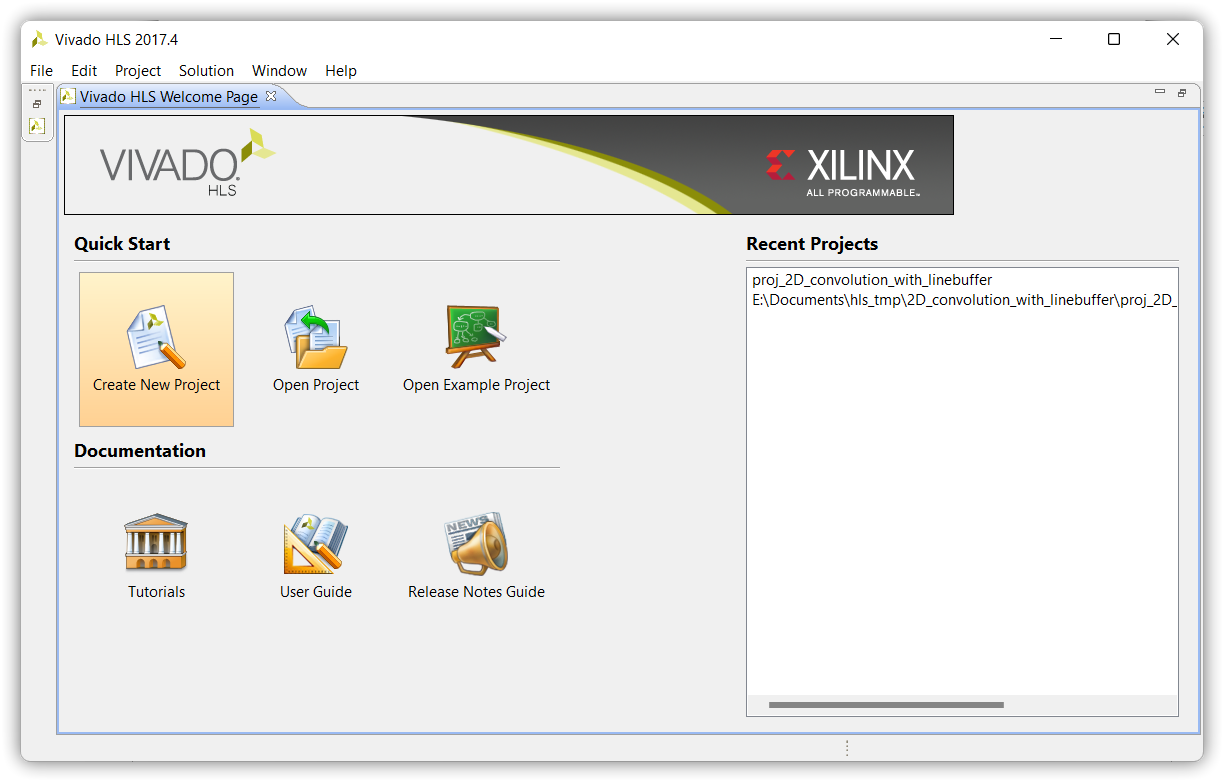
\includegraphics[width=.8\linewidth]{win/helloworld/welcome.png}
      \caption{欢迎界面}
      \label{fig:welcome}
    \end{figure}
    在创建我们需要的 Hello World 之前可以选择
    Open Example Project 查看并仿真、综合提供的示例代码。
    点击 Create New Project 创建新项目,
    可以看到如\cref{fig:new_project} 所示的界面,设置项目的名称和路径,
    项目名称设置为 \texttt{helloworld} 即可。
    需要注意的是项目会创建一个路径下的新文件夹,因此不需要为项目单独创建一个文件夹。
    接下来两步分别要求添加源代码和测试(testbench)代码,按照要求添加即可。
    此处我们可以先不添加,在创建完项目后单独新建。
    添加源代码时需要设置 top 模块的名称,设置其为 \texttt{helloworld}(此设置后续仍然可以更改)。
    最后,需要设置解决方案(solution)的名称,默认为 \texttt{solution1},我们也不对其进行修改。
    时钟周期(Clock Period)以及不确定度(Uncertainty)可以自行设置,不确定度可以空着使用默认值。
    在这个界面同时需要设置使用的芯片,简单起见,这里就选用了开发版(Board)Virtex-7 VC709 Evaluation Platform,
    这对于目前的例子影响不大,如\cref{fig:init_sol} 所示。
    \begin{figure}[h!]
      \centering
      \subfloat[创建新项目]{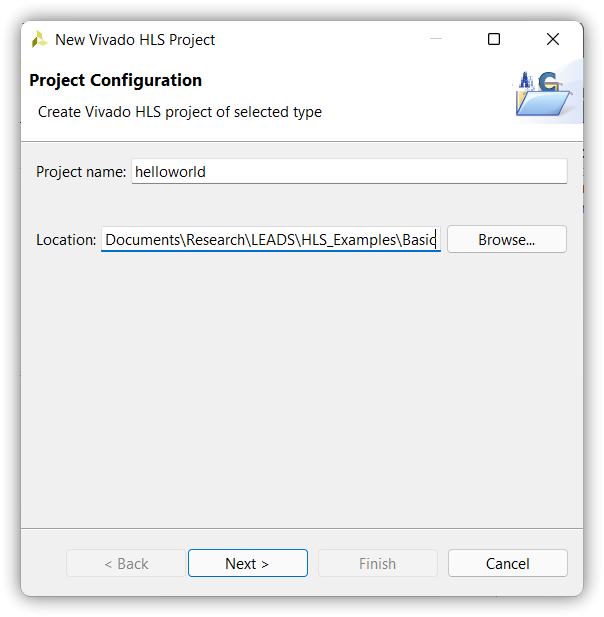
\includegraphics[width=.4\linewidth]{win/helloworld/new_project.png}\label{fig:new_project}}\quad
      \subfloat[设置解决方案等]{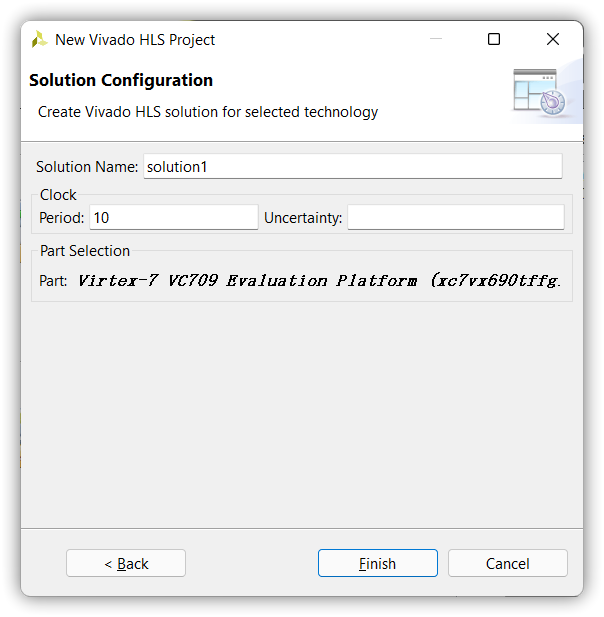
\includegraphics[width=.4\linewidth]{win/helloworld/init_sol.png}\label{fig:init_sol}}
      \caption{创建并设置新项目}
    \end{figure}

  \section{使用 C++ 进行模块设计}

    接着,我们就可以进行 C++ 的 \texttt{helloworld} 模块设计,
    在左侧 Explorer 框的 Includes、Sources 和 Test Bench 中分别添加头文件(\texttt{.h})、源文件(\texttt{.cpp})和测试文件(包括 \texttt{main} 函数的 \texttt{.cpp} 以及其他测试中运用到的文件,例如数据文件 \texttt{.dat} 等)。
    
    此处建议使用其他的文本编辑器编辑代码,这能够提供更加丝滑的 coding 体验,例如
    \begin{figure}[htbp]
      \centering
      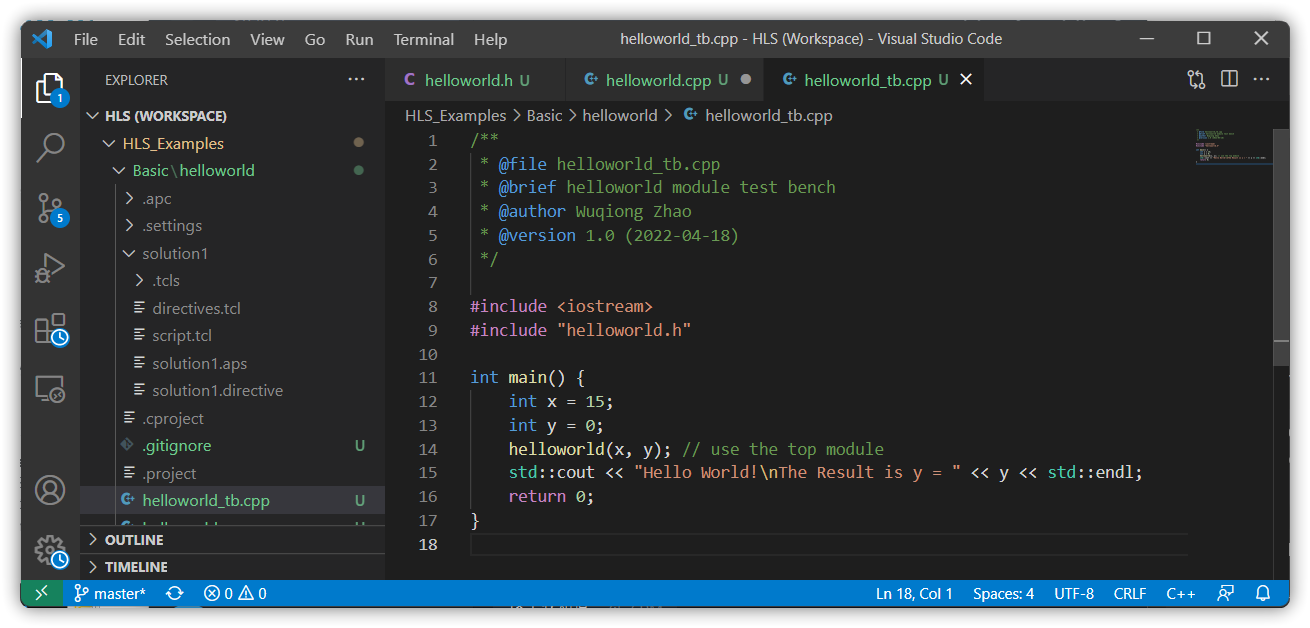
\includegraphics[width=.8\linewidth]{win/helloworld/vscode_edit.png}
      \caption{使用 VS Code 编辑 C++ 代码}
    \end{figure}

    忽略文件信息注释,主要的三个文件代码及解释如下。

    头文件 \texttt{helloworld.h} 申明了函数 \texttt{helloworld},
    这个函数返回值为空(\texttt{void}),
    而是使用了类似 Verilog 的输入输出模式:
    输入为 \texttt{int} 类型的变量 \texttt{a},采用传值的形式,对应 Verilog 中的 \texttt{input};
    输出为 \texttt{int\&} 类型的变量 \texttt{b},采用引用可以对其值进行修改,对应 Verilog 中的 \texttt{output}。
    \begin{warning}
      此处的函数及变量命名为了简便起见(且符合 C++ 命名习惯),没有按照 Verilog 规范进行。
      之后完整的示例中将会规范命名。
    \end{warning}
    \begin{lstlisting}[language=C++, title={helloworld.h}]
#ifndef _HELLOWORLD_H_
#define _HELLOWORLD_H_

/**
 * @brief helloworld module
 * @details right shift a one bit
 * @param a [in] integer
 * @param b [out] the shifted value
 */
void helloworld(int a, int& b);

#endif
    \end{lstlisting}
    
    \texttt{helloworld} 函数的实现则在 \texttt{helloworld.cpp} 中完成,
    内容非常简单,输出的 \texttt{b} 就是输入 \texttt{a} 逻辑右移一位的结果。
    \begin{lstlisting}[language=C++, title={helloworld.cpp}]
#include "helloworld.h"

void helloworld(int a, int& b) {
    b = a >> 1; // right shift one bit
}
    \end{lstlisting}

    函数功能的验证在 \texttt{helloworld\_tb.cpp} 中完成,包括了 \texttt{main} 函数。
    \begin{lstlisting}[language=C++, title={helloworld\_tb.cpp},morekeywords={std,cout,endl}]
#include <iostream>
#include "helloworld.h"

int main() {
    int x = 15;
    int y = 0;
    helloworld(x, y); // use the top module
    std::cout << "Hello World!\nThe Result is y = " << y << std::endl;
    return 0;
}
    \end{lstlisting}

  \section{CSim --- C++ 仿真测试}

    在上一个步骤完成 C++ 代码的书写,
    可以进行 C Simulation,其对应的按钮图标为“窗口框左下有一个绿三角”,即\cref{fig:C_simulation} 右上角的图标。
    \begin{figure}[htbp]
      \centering
      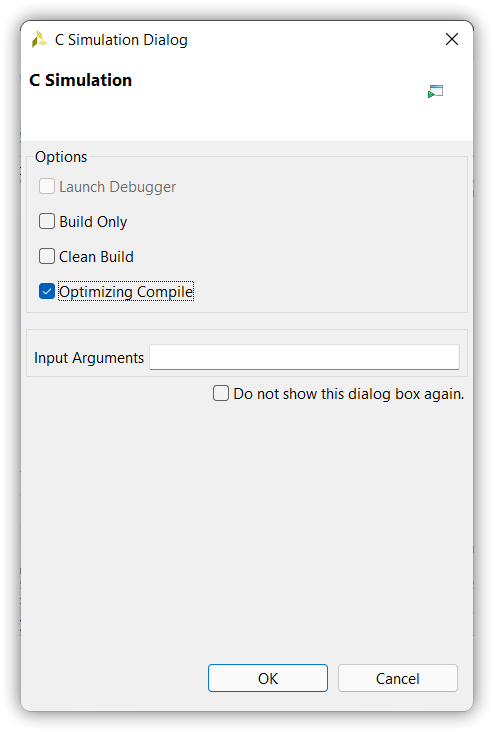
\includegraphics[width=.3\linewidth]{win/helloworld/C_simulation.png}
      \caption{CSim 设置}
      \label{fig:C_simulation}
    \end{figure}

    点击后会弹出\cref{fig:C_simulation} 的设置,四个选项分别表示调试(Debug 模式)、仅编译、清理编译和优化编译(Release 模式)。
    此处我们选择优化编译。
    \begin{tip}[Linux 系统功能]
      如果在 Linux 系统上,还可以选择 C++ 编译器为 GCC 或 Clang。
    \end{tip}
    Input Argument 是 C++ 编译时的命令行选项,例如增加 \texttt{-std=c++03} 可以设置 C++ 编译标准为 C++03。
    如果编译成功,我们会得到如\cref{fig:csim_result} 中的结果,可以看到,输出结果 \texttt{7} 正是我们预期的。
    % 另外可以观察到多出了 \texttt{csim} 文件夹。
    \begin{figure}[htbp]
      \centering
      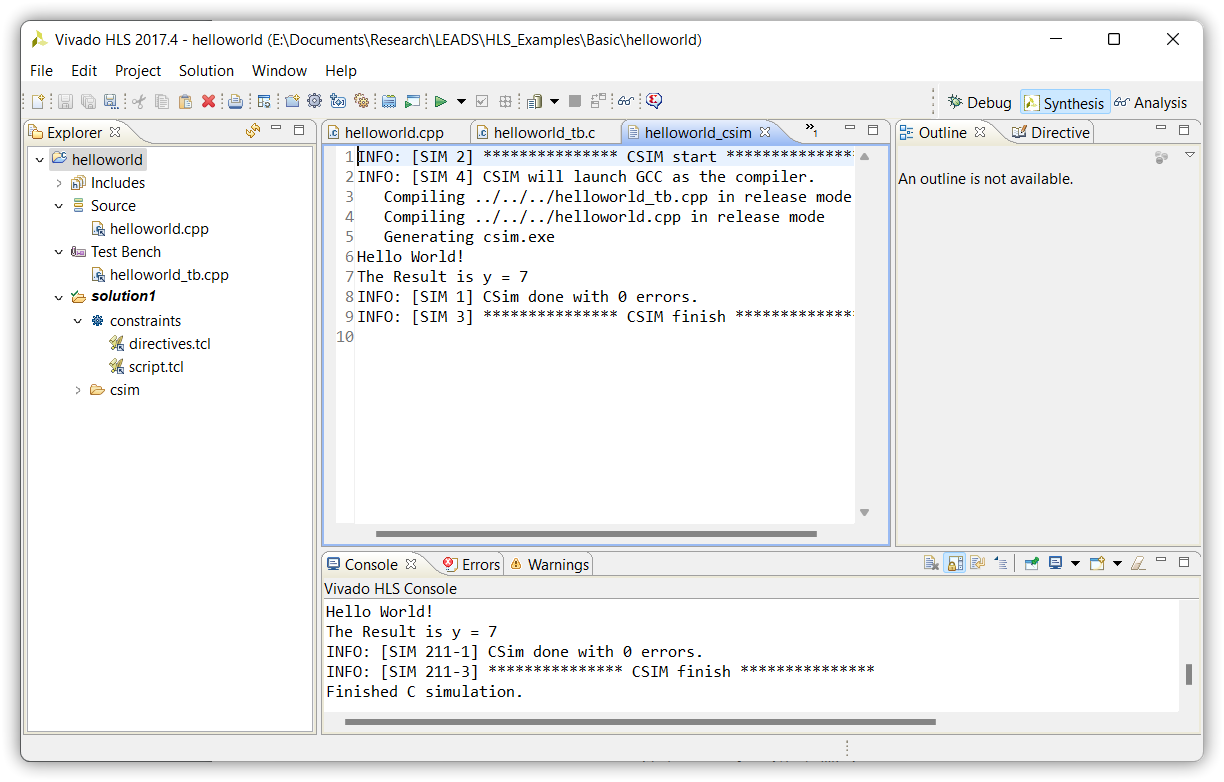
\includegraphics[width=.8\linewidth]{win/helloworld/csim_result.png}
      \caption{CSim 结果}
      \label{fig:csim_result}
    \end{figure}

  \section{Syn --- 综合}

    完成 C 仿真后,点击 CSim 右边绿箭头进行综合,可以得到\cref{fig:syn_result} 中的结果。
    中间页面给出了综合报告,对于各项资源的利用给出了分析。
    另外,点击窗口右上角的 Analysis,可以查看其他例如时序的分析结果。
    \begin{figure}[htbp]
      \centering
      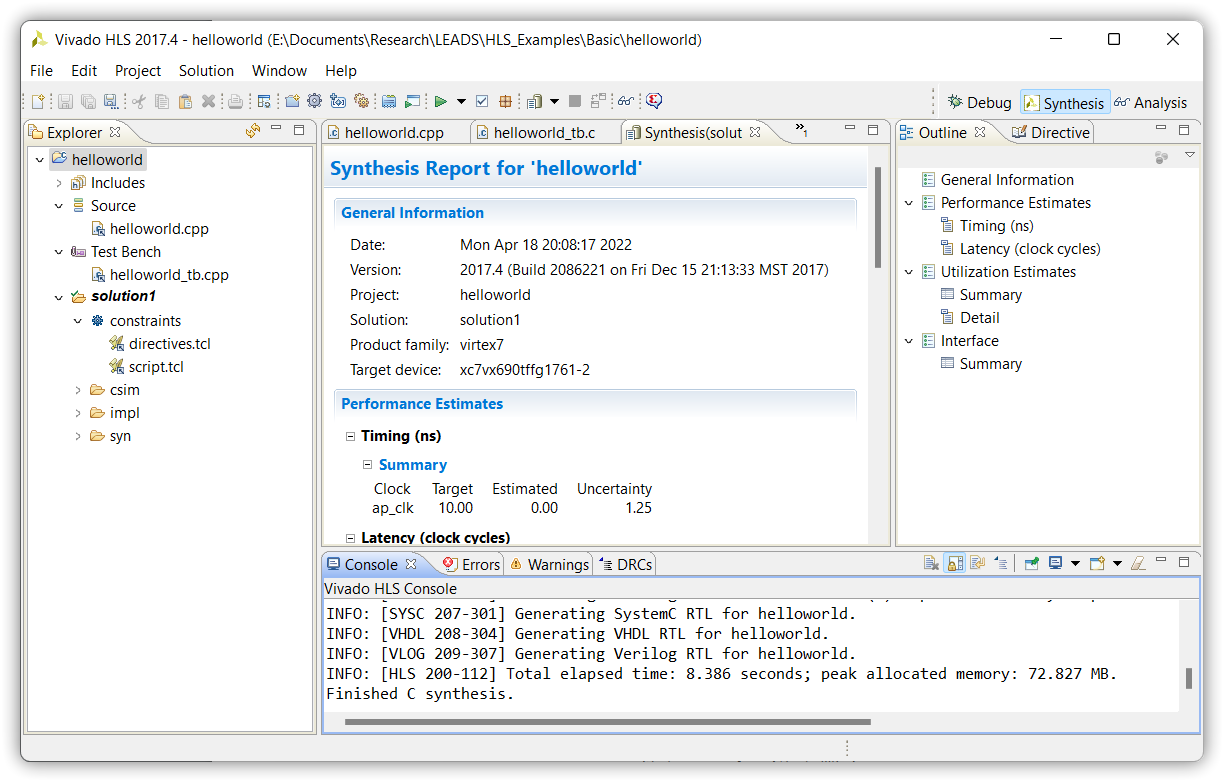
\includegraphics[width=.8\linewidth]{win/helloworld/syn_result.png}
      \caption{Syn 结果}
      \label{fig:syn_result}
    \end{figure}
    \begin{warning}
      Syn 时使用的逻辑与 CSim 和 CoSim 不一样,所以经常会出现 Syn 成功但是 CSim 和(尤其)CoSim 不成功的情况,
      因此不能过于相信 Syn 的正确性。
    \end{warning}

  \section{CoSim --- RTL/C 联合仿真}

    在正式完成之前,还需要进行最后的验证——RTL 的结果和 C 仿真结果是否一致,
    因此,需要 RTL/C 联合仿真(CoSim)。
    其按钮图标为 Syn 右边一个“窗口中带一个钩”,即\cref{fig:C_RTL_cosim} 右上角的图标。
    \begin{figure}[htbp]
      \centering
      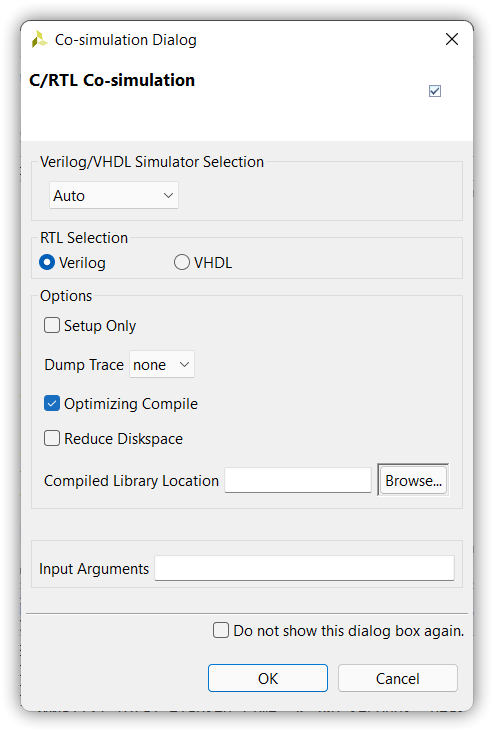
\includegraphics[width=.3\linewidth]{win/helloworld/C_RTL_cosim.png}
      \caption{CoSim 设置}
      \label{fig:C_RTL_cosim}
    \end{figure}

    此处,我们选择基于 Verilog 的 RTL 综合(也可以选择 VHDL),并且勾选优化编译与之前 CSim 一致。
    类似地,这里也可以设置对应的 Input Arguments。
    \begin{tip}[Linux 系统功能]
      与 CSim 中类似,CoSim 也可以选择编译器为 GCC 或 Clang。(Ubuntu 20 上 CSim 可以通过,但是 CoSim 就会遇到 linker error。鉴于这些不确定性,不建议在 Linux 系统上展开这些工作,或严格按照 Vivado 支持的系统配置。)
    \end{tip}

    CoSim 的结果如\cref{fig:cosim_result} 所示,给出了 Verilog 测试的通过。
    如果代码更复杂,可以看到对应的 Latency 和 Interval 值。
    \begin{figure}[htbp]
      \centering
      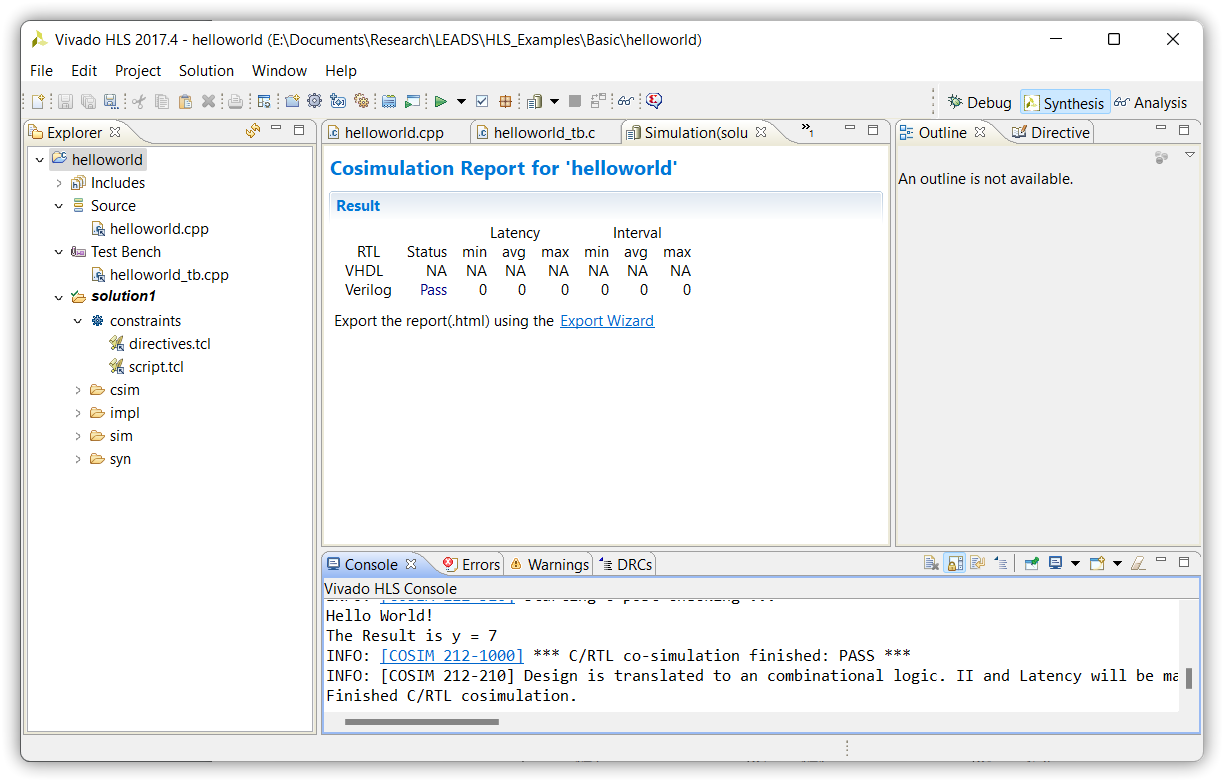
\includegraphics[width=.8\linewidth]{win/helloworld/cosim_result.png}
      \caption{CoSim 结果}
      \label{fig:cosim_result}
    \end{figure}

  \section{Exp --- 导出 IP 核}

    在通过 CoSim 后,基本可以认定设计正确了,
    此时可以导出 IP 核(当然可以在窗口中设置为其他形式),
    点击 CoSim 右侧“棕色上有十字”的图标,跳出\cref{fig:export_IP} 窗口进行设置。
    \begin{figure}[htbp]
      \centering
      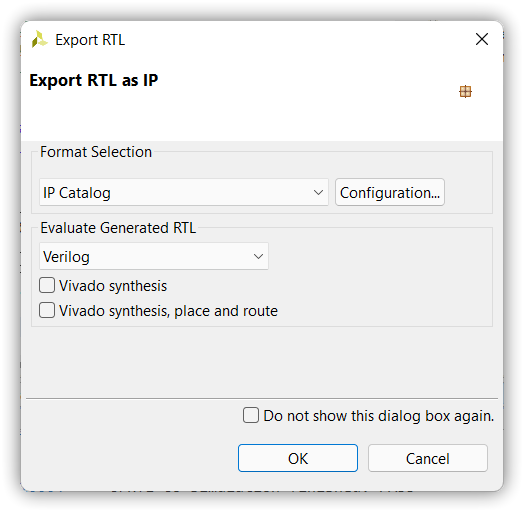
\includegraphics[width=.3\linewidth]{win/helloworld/export_IP.png}
      \caption{导出设置}
      \label{fig:export_IP}
    \end{figure}
    \begin{tip}[Vivado HLS Bug]
      此处会提示导出失败。而错误的原因实际上是 Xilinx Vivado 的一个 bug。
      Bug 的主要原因是 HLS 定义的 \texttt{ip\_version} 采用格式 \texttt{YYMMDDHHMM} 是一个有符号 32 位数,
      因此从2022年1月1日起均会导出失败。
      需要在\href{https://support.xilinx.com/s/article/76960?language=en_US}{Xilinx 网站}下载对应的补丁。
      然后根据要求运行对应的 Python 代码修复问题。
    \end{tip}
    
    完成之后,我们就可以在 \texttt{impl/ip} 文件夹下找到生成的 zip 压缩的 IP 核。
    \texttt{impl} 文件夹下还会提供原始的 Verilog 代码,根据 Xilinx 官方描述,那些代码进攻测试使用,不代表最后导出的结果。

  \section{测试导出的 IP 核}

    \subsection{导入 IP 核}

      现在已经完成了所有的 HLS 设计工作,不过仍然可以验证我们导出的 \texttt{helloworld} IP 核的效果。
      在 IP Catalog 中新增 Repository,文件夹中加入解压后的 IP 核,得到如\cref{fig:manage_ip} 的效果。
      \begin{figure}[htbp]
        \centering
        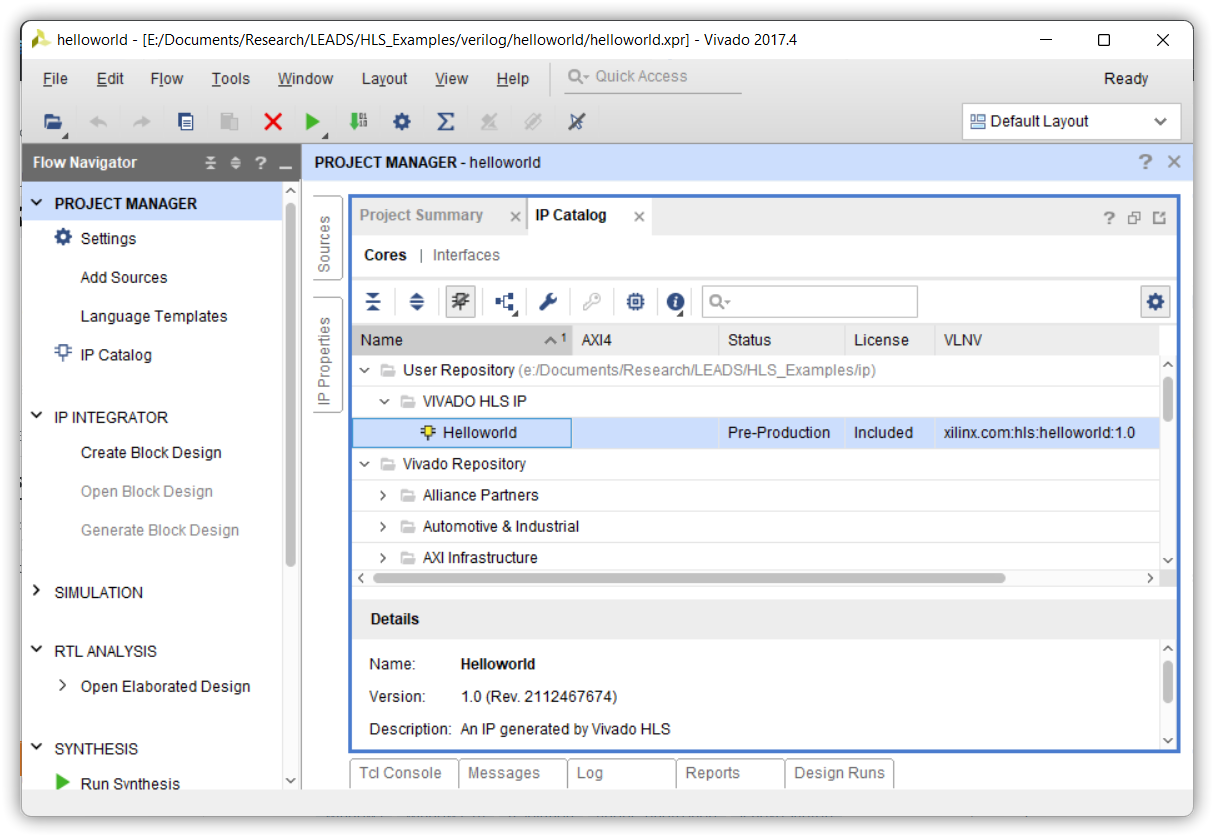
\includegraphics[width=.8\linewidth]{win/helloworld/manage_ip.png}
        \caption{管理 IP 核}
        \label{fig:manage_ip}
      \end{figure}

      双击使用 IP 核,并复制其中的 template 内容进入下一部分需要完成的 Test Bench 文件。

    \subsection{Test Bench 测试}


      增加 Test Bench 文件 \texttt{helloworld\_ip\_tb.v},模块名为 \texttt{HELLOWORLD\_IP\_TB}。
      其中创建的 \texttt{HELLO\_WORLD} instance 名为 \texttt{Uhelloworld}。
      \begin{lstlisting}[style={v}, title={helloworld\_ip\_tb.v}]
`timescale 1ns / 1ps

module HELLOWORLD_IP_TB();

    parameter   CYC         = 10;
    parameter   DELAY       = 1;
    parameter   START_TIME  = CYC;
    parameter   FINISH_TIME = 40 * CYC;
    reg         Clk = 0;

    // Input
    reg         Start       = 0;
    reg  [31:0] Data_in     = 0;
    // Output
    wire        Vld;
    wire [31:0] Data_out;
        
    HELLO_WORLD Uhelloworld (
        .b_ap_vld (Vld     ),  // output wire b_ap_vld
        .ap_start (Start   ),  // input wire ap_start
        .ap_done  (        ),  // output wire ap_done
        .ap_idle  (        ),  // output wire ap_idle
        .ap_ready (        ),  // output wire ap_ready
        .a        (Data_in ),  // input wire [31 : 0] a
        .b        (Data_out)   // output wire [31 : 0] b
    );

    initial begin
        #START_TIME  Start <= 1'b1;
        #FINISH_TIME $finish;
    end
    
    always #CYC Clk = ~Clk;
    
    always @(posedge Clk) begin
        #DELAY Data_in = Data_in + 1;    // increment one each clock
        #DELAY $display("Data Out: %b", Data_out); // display result
    end
    
endmodule // of HELLOWORLD_IP_TB
      \end{lstlisting}

      行为测试的结果如\cref{fig:behavioral_sim} 所示。
      \begin{figure}[htbp]
        \centering
        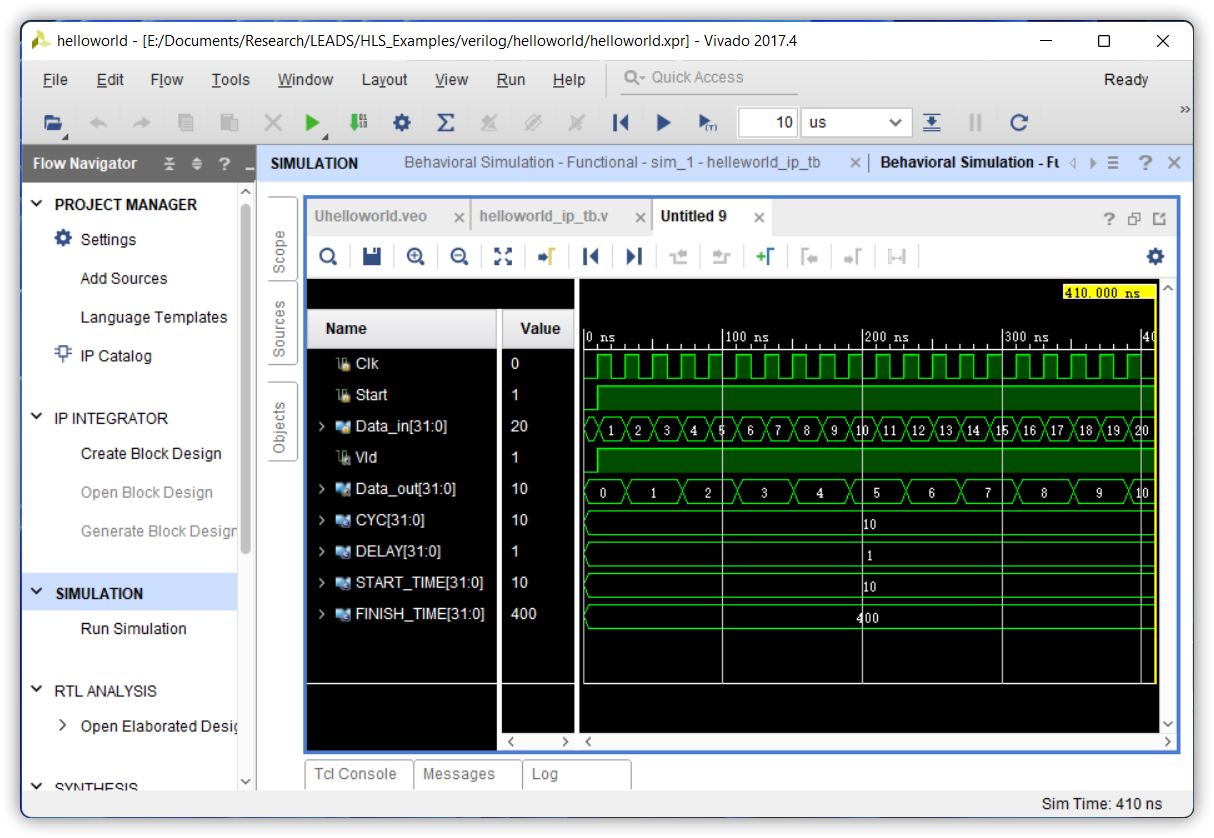
\includegraphics[width=.8\linewidth]{win/helloworld/behavioral_sim.png}
        \caption{行为仿真测试}
        \label{fig:behavioral_sim}
      \end{figure}

      我们也可以对其做 RTL 级分析,如\cref{fig:RTL_result} 所示。
      \begin{figure}[htbp]
        \centering
        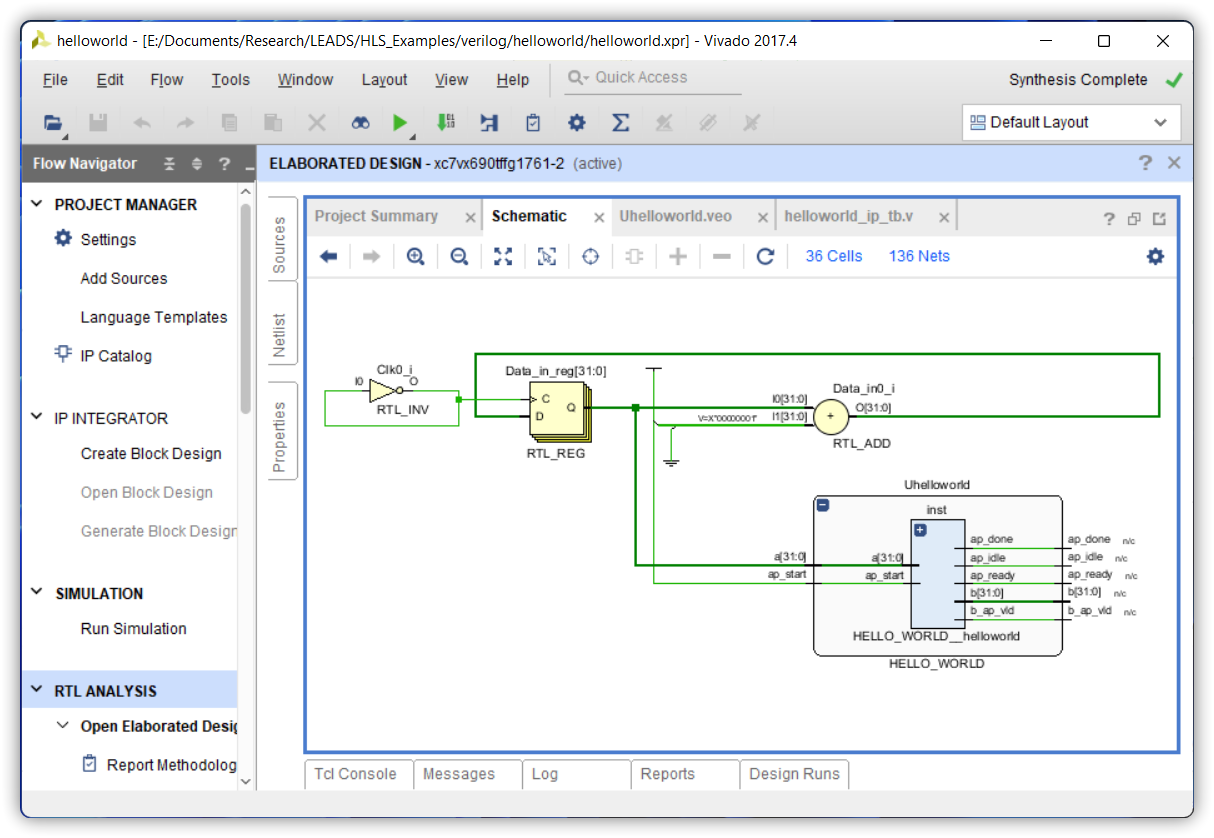
\includegraphics[width=.8\linewidth]{win/helloworld/RTL_result.png}
        \caption{RTL 级电路}
        \label{fig:RTL_result}
      \end{figure}    

\chapter{FFT}

\end{document}
\endinput
